%\VignetteIndexEntry{Exercise 02 from Seminar III: R/Bioconductor}
%\VignetteDepends{}
%\VignetteKeywords{R, Bioconductor}
%\VignettePackage{SIII: R/Bioc}
\documentclass[letterpaper,12pt]{article}

%%%%%%%%%%%%%%%%%%%%%%%% Standard Packages %%%%%%%%%%%%%%%%%%%%%%%%%%%%%%%%%%%%%%%%%%
%\usepackage{epsfig}
%\usepackage{graphicx}
%\usepackage{graphics}
%\usepackage{amssymb}
%\usepackage{amsmath}
%\usepackage{mathrsfs}
%\usepackage{caption}
%\usepackage{comment}
\usepackage{fancyvrb}
\usepackage{fancyhdr}

\usepackage[a4paper]{geometry}
\usepackage{hyperref,graphicx}

%\usepackage[spanish]{babel}
%\selectlanguage{spanish}
%\usepackage[utf8]{inputenc}

%%%%%%%%%%%%%%%%%%%%%% some personal commands %%%%%%%%%%%%%%%%%%%%%%%%%%%%%%%%%%%%%%%%%%%%
\newcommand{\pl}[1]{\texttt{#1}}
\newcommand{\myurlshort}[2]{\href{http://#1}{{\textsf{#2}}}}

%%%%%%%%%%%%%%%%%%%%%% headers and footers %%%%%%%%%%%%%%%%%%%%%%%%%%%%%%%%%%%%%%%%%%%%
\pagestyle{fancy} 
\renewcommand{\footrulewidth}{\headrulewidth}

%%%%%%%%%%%%%%%%%%%%%%%%% bibliography  %%%%%%%%%%%%%%%%%%%%%%%%%%%%%%%%%%%%%%%%%%%%%%%
\bibliographystyle{plainnat}

%%%%%%%%%%%%%%%%%%%%%%%%% sweave options  %%%%%%%%%%%%%%%%%%%%%%%%%%%%%%%%%%%%%%%%%%%%%%%




%%%%%%%%%%%%%%%%%%%%%%% opening %%%%%%%%%%%%%%%%%%%%%%%%%%%%%%%%%%%%
\title{\textbf{Seminar III: \texttt{R}/\texttt{Bioconductor}\\ \small August-December 2009}}
\author{Leonardo Collado Torres\\[1em]Bachelor in Genomic Sciences (LCG),\\ UNAM, Cuernavaca, Mexico\\[1em]\texttt{lcollado@lcg.unam.mx}\\[1em]\url{http://www.lcg.unam.mx/~lcollado/}}

\usepackage{Sweave}
\begin{document}
\maketitle

\medskip
\noindent{\small\textbf{Assistants:} Alejandro Reyes \pl{areyes@lcg.unam.mx}, Jos\'e Reyes \pl{jreyes@lcg.unam.mx} and V\'ictor Moreno \pl{jmoreno@lcg.unam.mx}}

\medskip
\noindent{\small\textbf{Note:} Questions through the \myurlshort{foros.nnb.unam.mx/viewforum.php?f=111}{forum} please. Those who are not from the sixth LCG generation send us an email so we can register you on the forum.}

\medskip
\begin{abstract}
With the following exercises you'll practice creating some advanced plots. You'll have to explain every plot.
\end{abstract}

\section{lattice}
\begin{Schunk}
\begin{Sinput}
> t1 <- read.csv("http://www.lcg.unam.mx/~lcollado/B/data/SuppTable01_kogenome6_double_end-clone_1132_742.csv", 
+     header = T)
> t2 <- read.csv("http://www.lcg.unam.mx/~lcollado/B/data/SuppTable06_nsSnp_AK1.csv", 
+     header = T)
> library(lattice)
> library(plotrix)
\end{Sinput}
\end{Schunk}
  \begin{enumerate}
  \item Using our object \pl{t1}, create a histogram of the BAC sizes with one panel per chromosome. With this plot we notice that mostly all the chromosomes have a tight BAC size distribution.
\begin{Schunk}
\begin{Sinput}
> print(histogram(~bac_size | chrNo, data = t1))
\end{Sinput}
\end{Schunk}
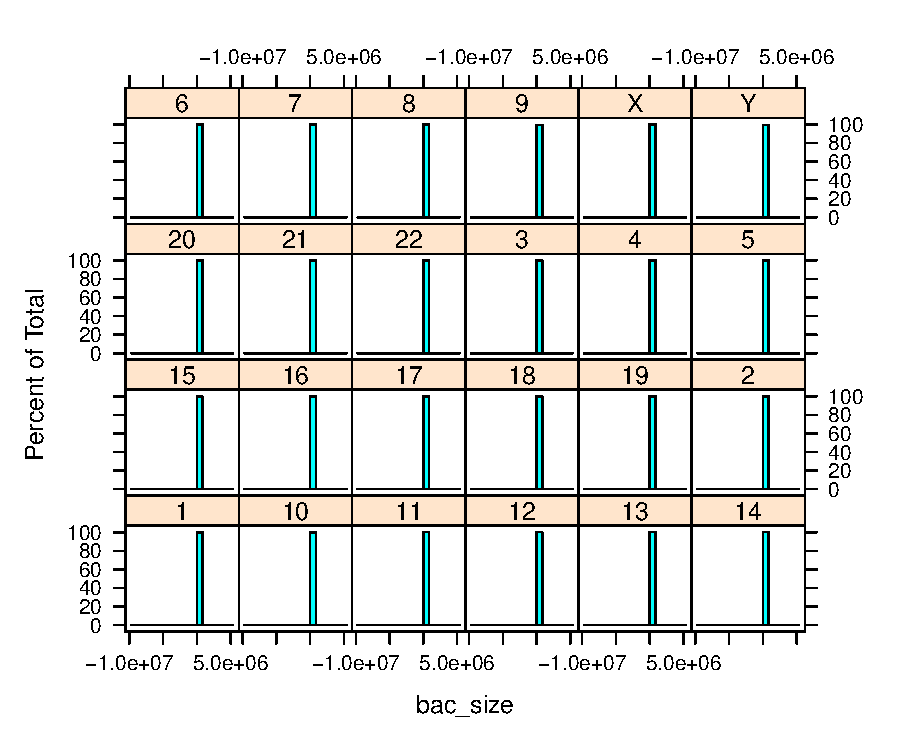
\includegraphics{plots/fig-002}
  \item With the object \pl{t2} from class, first normalize the position variable per chromosome (use tapply to find out the max values per chromosome). Then create density plots for your normalized position variable. Every chromosome has to have its own panel. Suprinsingly, chromosome Y only has one data point, and some are quite skewed such as chromosome 17.
\begin{Schunk}
\begin{Sinput}
> max <- tapply(t2$position, t2$chr, max)
> t2b <- t2
> for (i in 1:length(max)) {
+     pos <- which(t2b$chr %in% names(max[i]))
+     t2b$position[pos] <- t2b$position[pos]/max[i]
+ }
> print(densityplot(~position | chr, data = t2b))
\end{Sinput}
\end{Schunk}
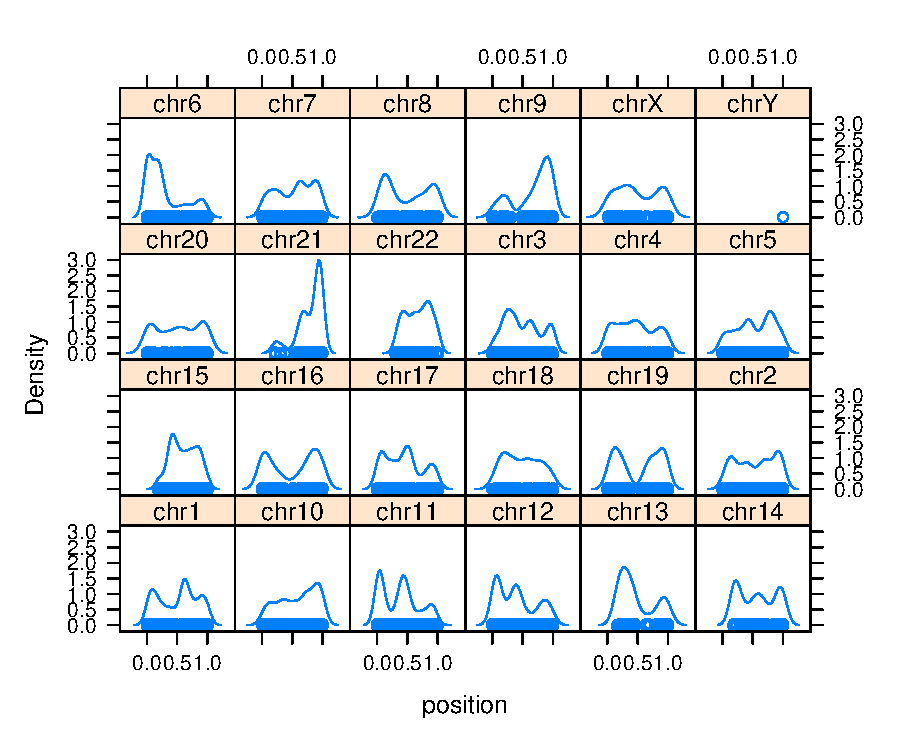
\includegraphics{plots/fig-003}
  \item For chromosomes X and Y, and using the normalized position variable, make a densityplot grouping the information by the reference allele. For each chromosome, separate the data by the AK1.allele variable\footnote{Remember that you can use more than 1 factor}. Your resulting plot should have 8 panels. With this graph we notice things like for chr X where most cases where the AK1.allele variable is a C, the reference allele variable is a T; and you find them on most of the chromosome except on some gaps visible with the data points.
\begin{Schunk}
\begin{Sinput}
> pos <- which(t2b$chr %in% c("chrX", "chrY"))
> print(densityplot(~position | chr * AK1.allele, groups = reference.allele, 
+     data = t2b, subset = pos, auto.key = T))
\end{Sinput}
\end{Schunk}
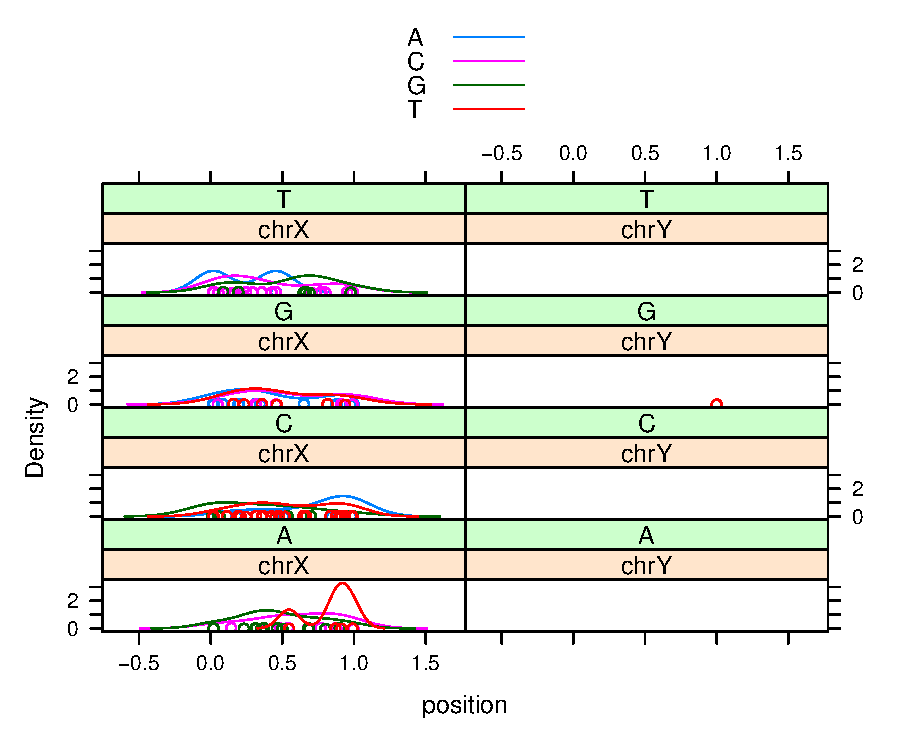
\includegraphics{plots/fig-004}
  \item (Optional) Check out the \pl{latticeExtra} package and make a plot with one of its functions.
  \end{enumerate}

\section{plotrix}
  \begin{enumerate}
  \item Using the original \pl{t2} object, plot for every chromosome the mean position with error bars. We did something very similar with \pl{t1} on class. In general, the error bars are small except for chromsomes such as the 23rd one we plot.
\begin{Schunk}
\begin{Sinput}
> means <- tapply(t2$position, t2$chr, mean)
> err <- tapply(t2$position, t2$chr, std.error)
> plotCI(1:24, means, err, col = "red", scol = "blue", las = 2, 
+     main = "Position per chr with error bars")
\end{Sinput}
\end{Schunk}
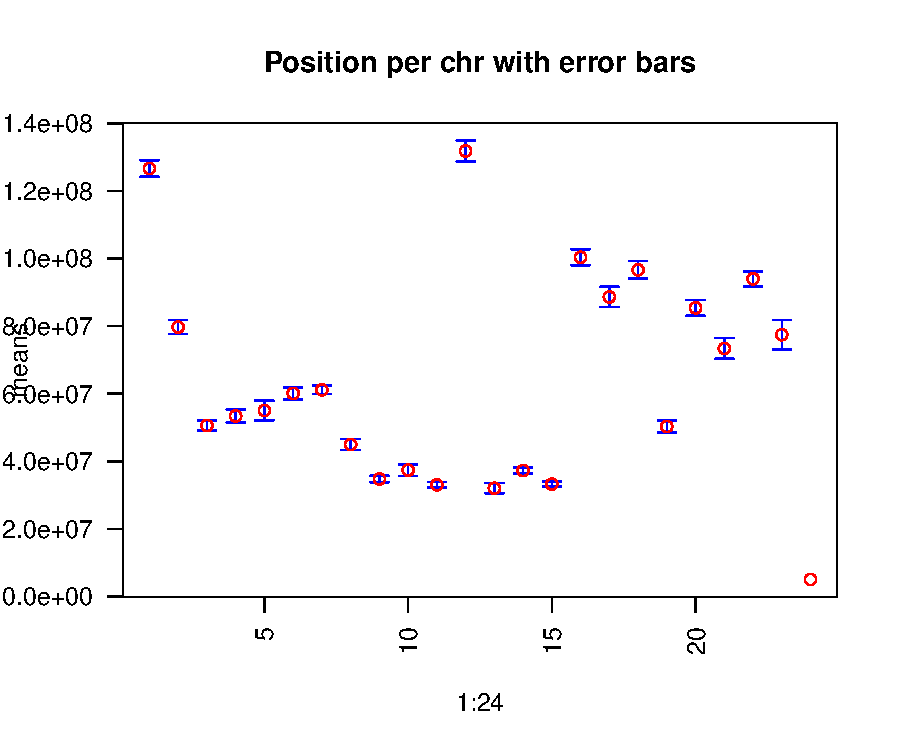
\includegraphics{plots/fig-005}
  \item Create a bar plot with the table information for the following data. With this plot, well, we can see the data values and the bars on one plot :)
\begin{Schunk}
\begin{Sinput}
> df <- data.frame(G1 = c(25, 5, 20), G2 = c(30, 6, 22), G3 = c(40, 
+     6, 18))
> df
\end{Sinput}
\begin{Soutput}
  G1 G2 G3
1 25 30 40
2  5  6  6
3 20 22 18
\end{Soutput}
\end{Schunk}
\begin{Schunk}
\begin{Sinput}
> barp(df, ylab = "Values", names.arg = colnames(df), col = 1:3)
> addtable2plot(0.45, 30, df, bty = "o", display.rownames = TRUE, 
+     hlines = TRUE, title = "Data in table format")
\end{Sinput}
\end{Schunk}
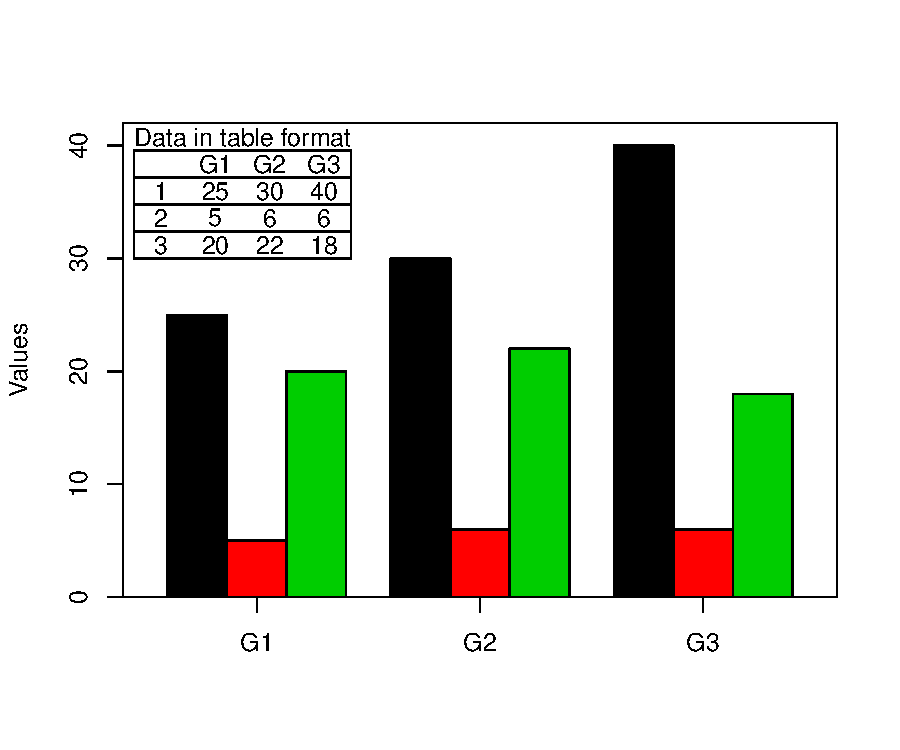
\includegraphics{plots/fig-007}
  \item (Optional) With whichever data you want, create an interesting plot using hierobarp. Don't use the default examples. 
  \end{enumerate}


\end{document}
